\chapter{理论基础}

\section{A理论}

\begin{figure}[htbp]
    \centering
    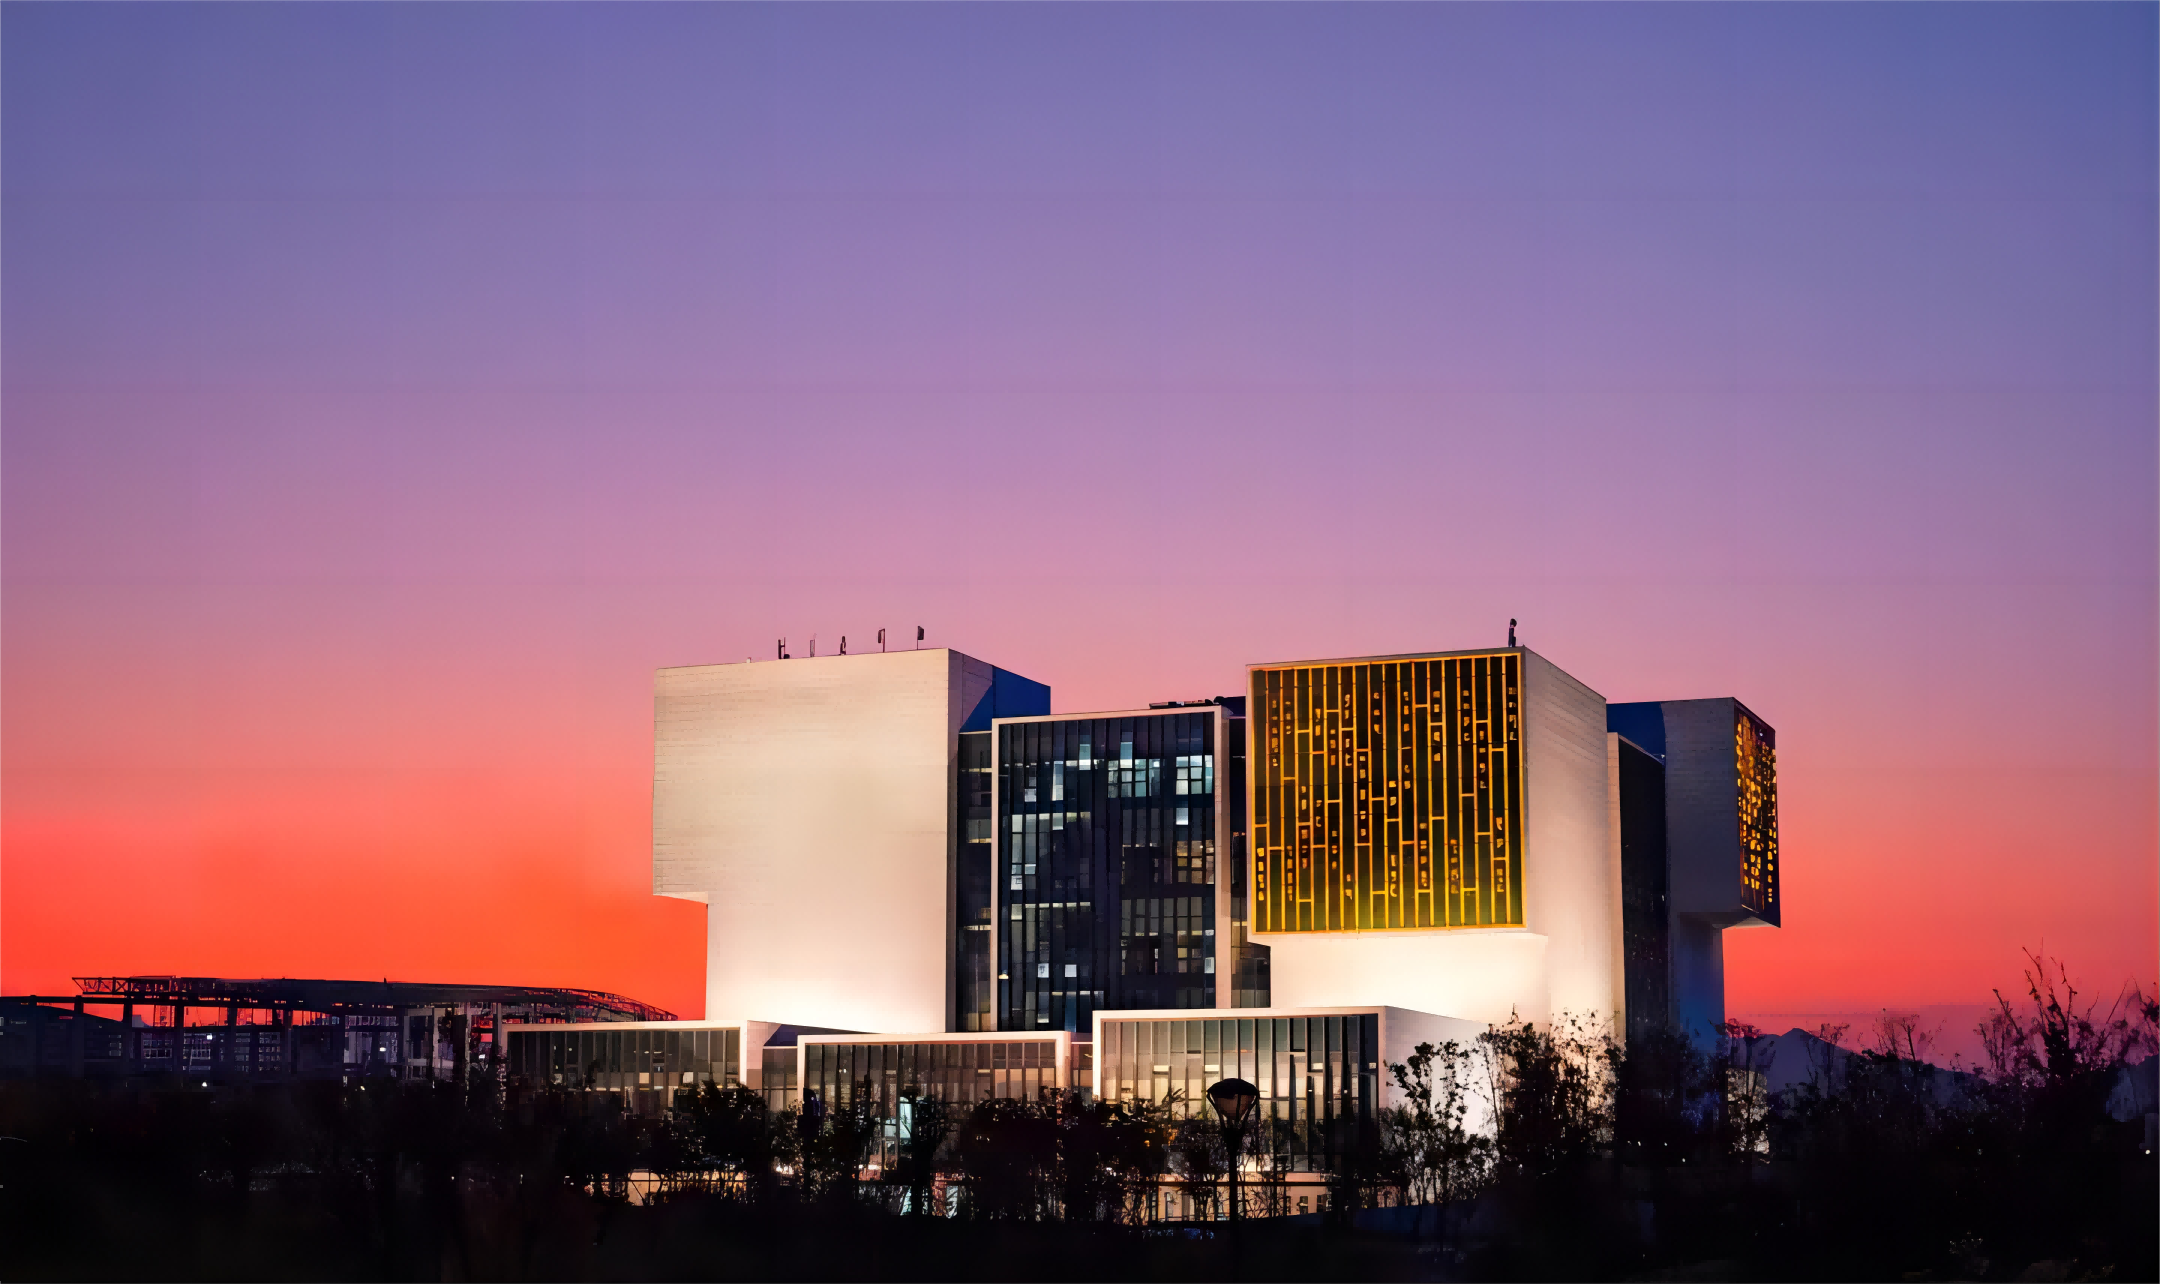
\includegraphics[width=0.7\textwidth]{testimage0.png}
    \caption{山东大学(青岛校区)博物馆外景图。}
    \label{fig:testimage0}
\end{figure}
\vspace{10pt}

这是\figref{fig:testimage0}。

\section{B理论}

\begin{figure}[htbp]
    \centering
    \subfloat[]{
        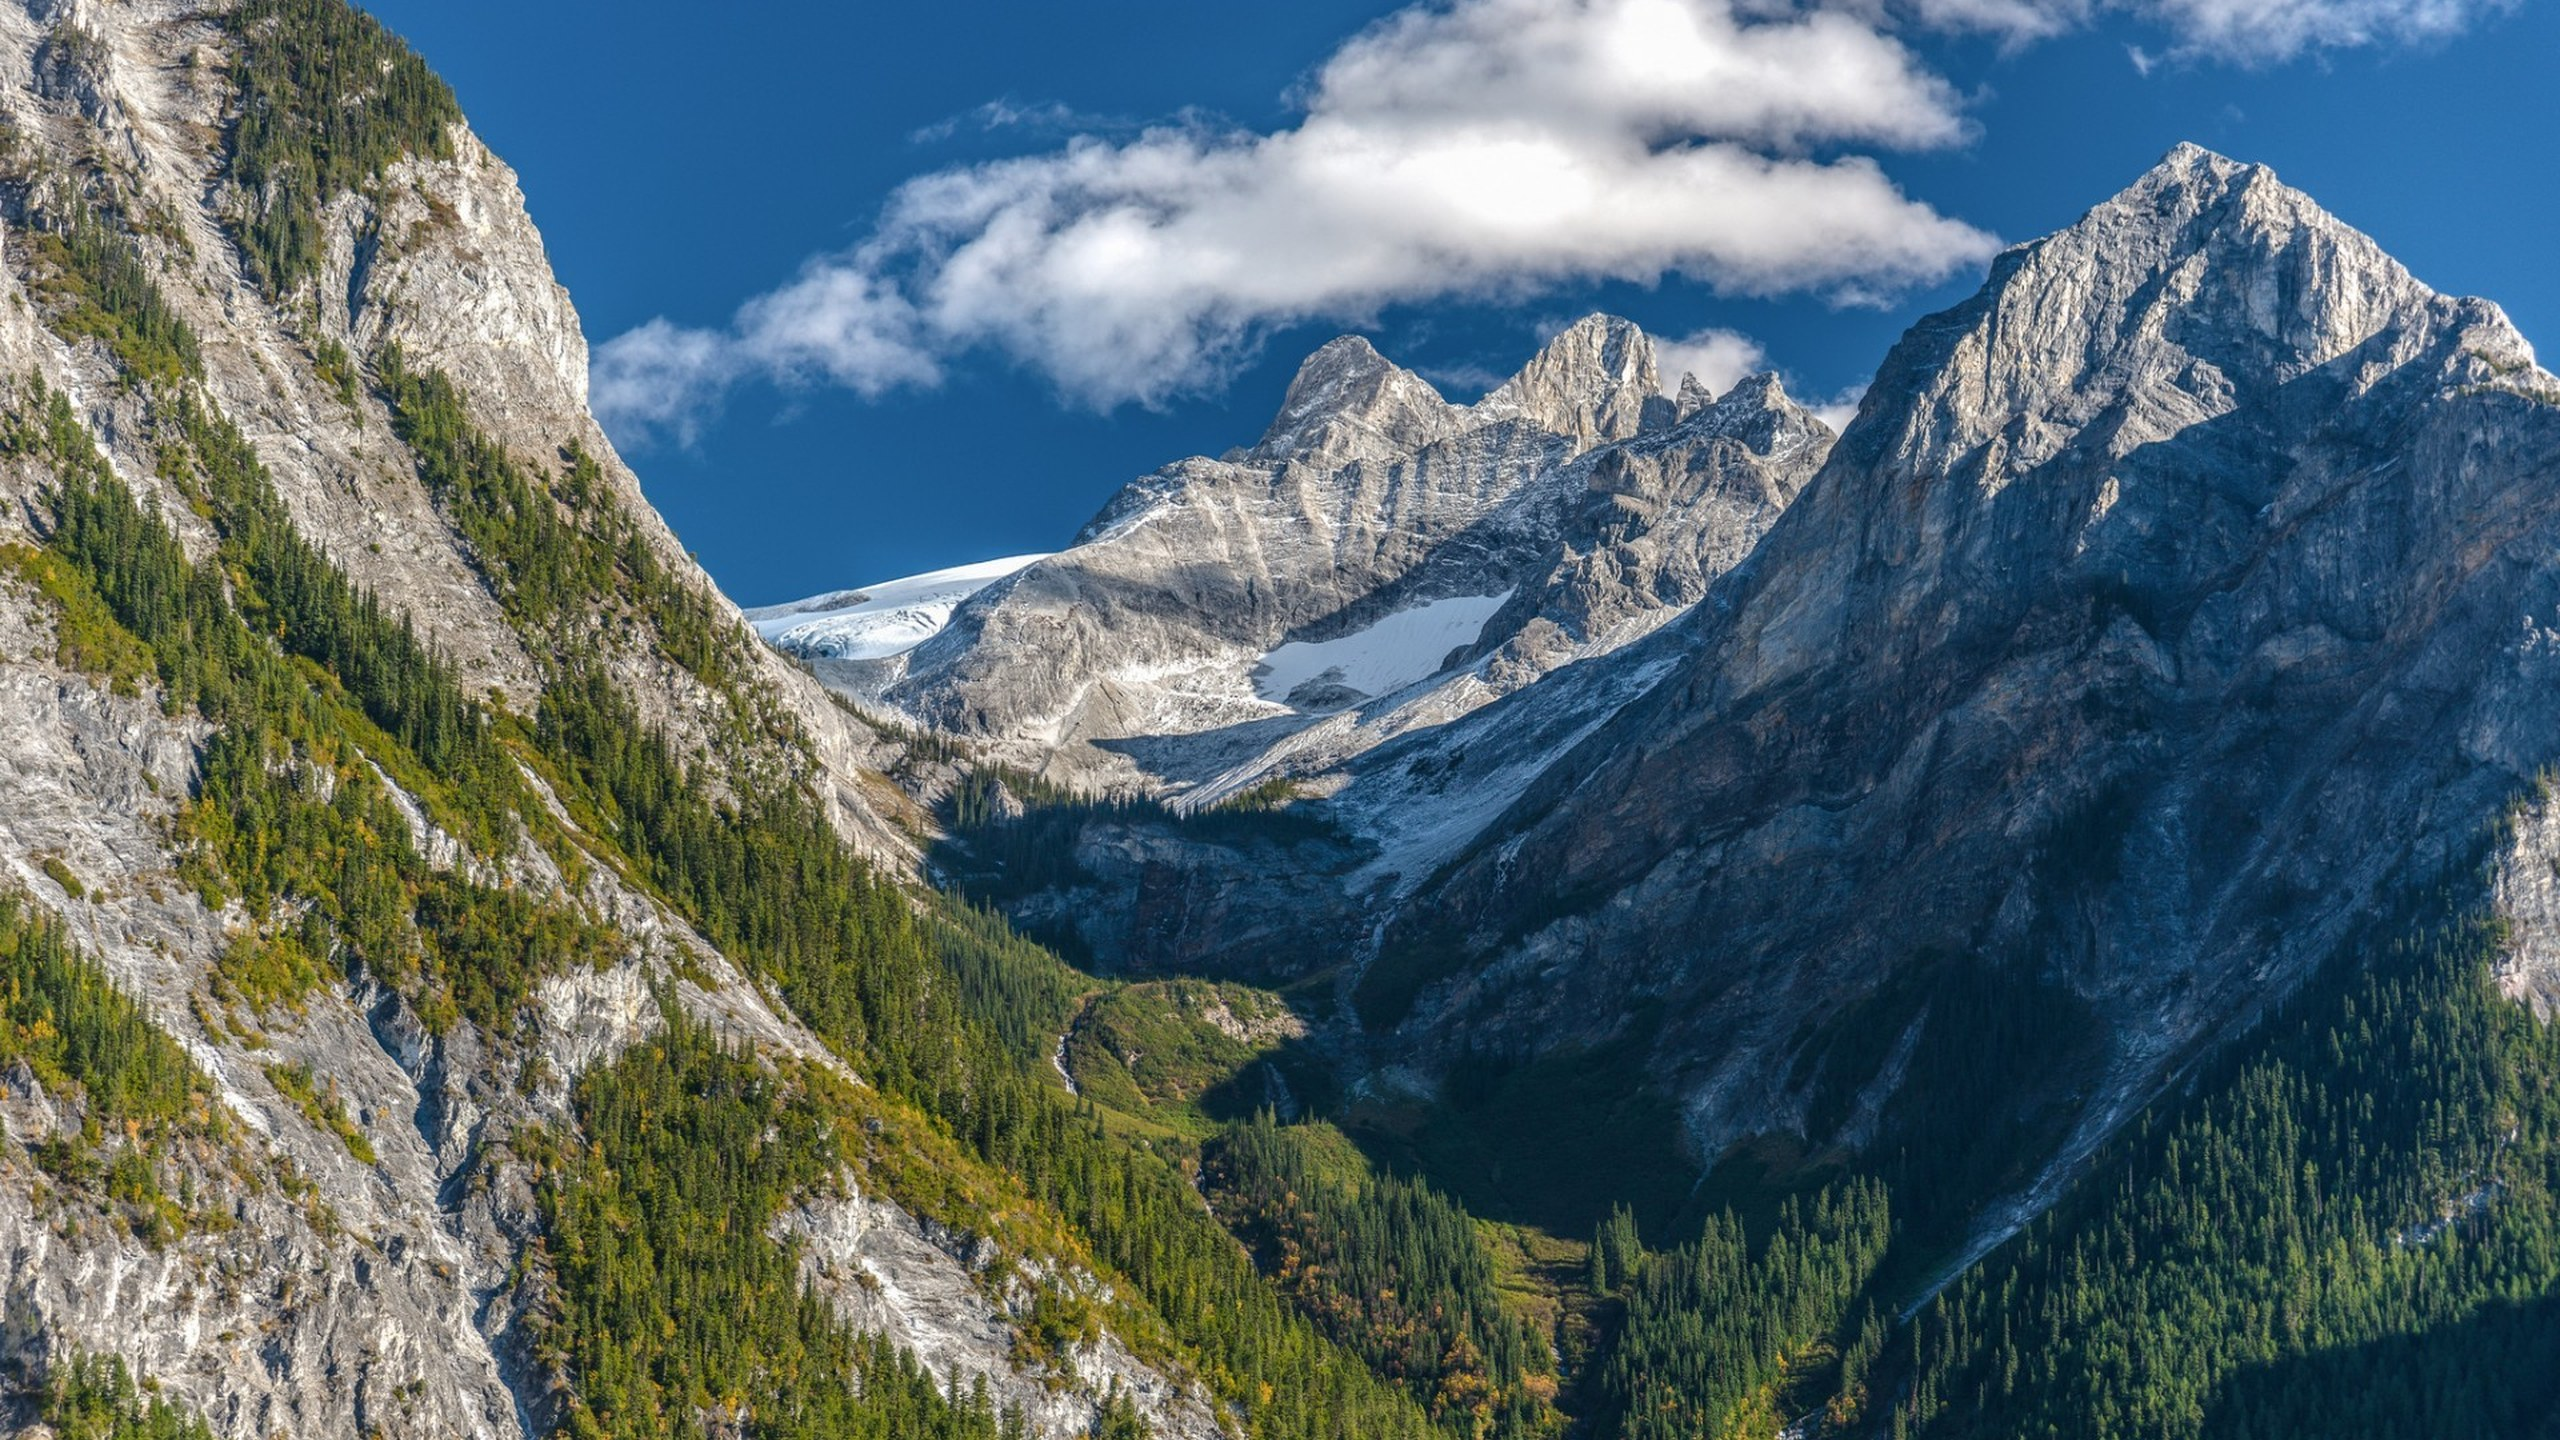
\includegraphics[width=0.48\textwidth]{testimage1.jpg}
        \label{subfig:testimage1}
    }
    \hfill
    \subfloat[]{
        
\includegraphics[width=0.48\textwidth]{testimage2.jpg}
        \label{subfig:testimage2}
    }
    \caption{这是一组风景图。(a)风景图1;(b)风景图2。}
    \label{fig:group1}
\end{figure}
\vspace{10pt}

这是\subfigref{subfig:testimage1},这是\subfigref{subfig:testimage2},这是\figref{fig:group1}。

\begin{figure}[htbp]
    \centering
    \subfloat[]{
        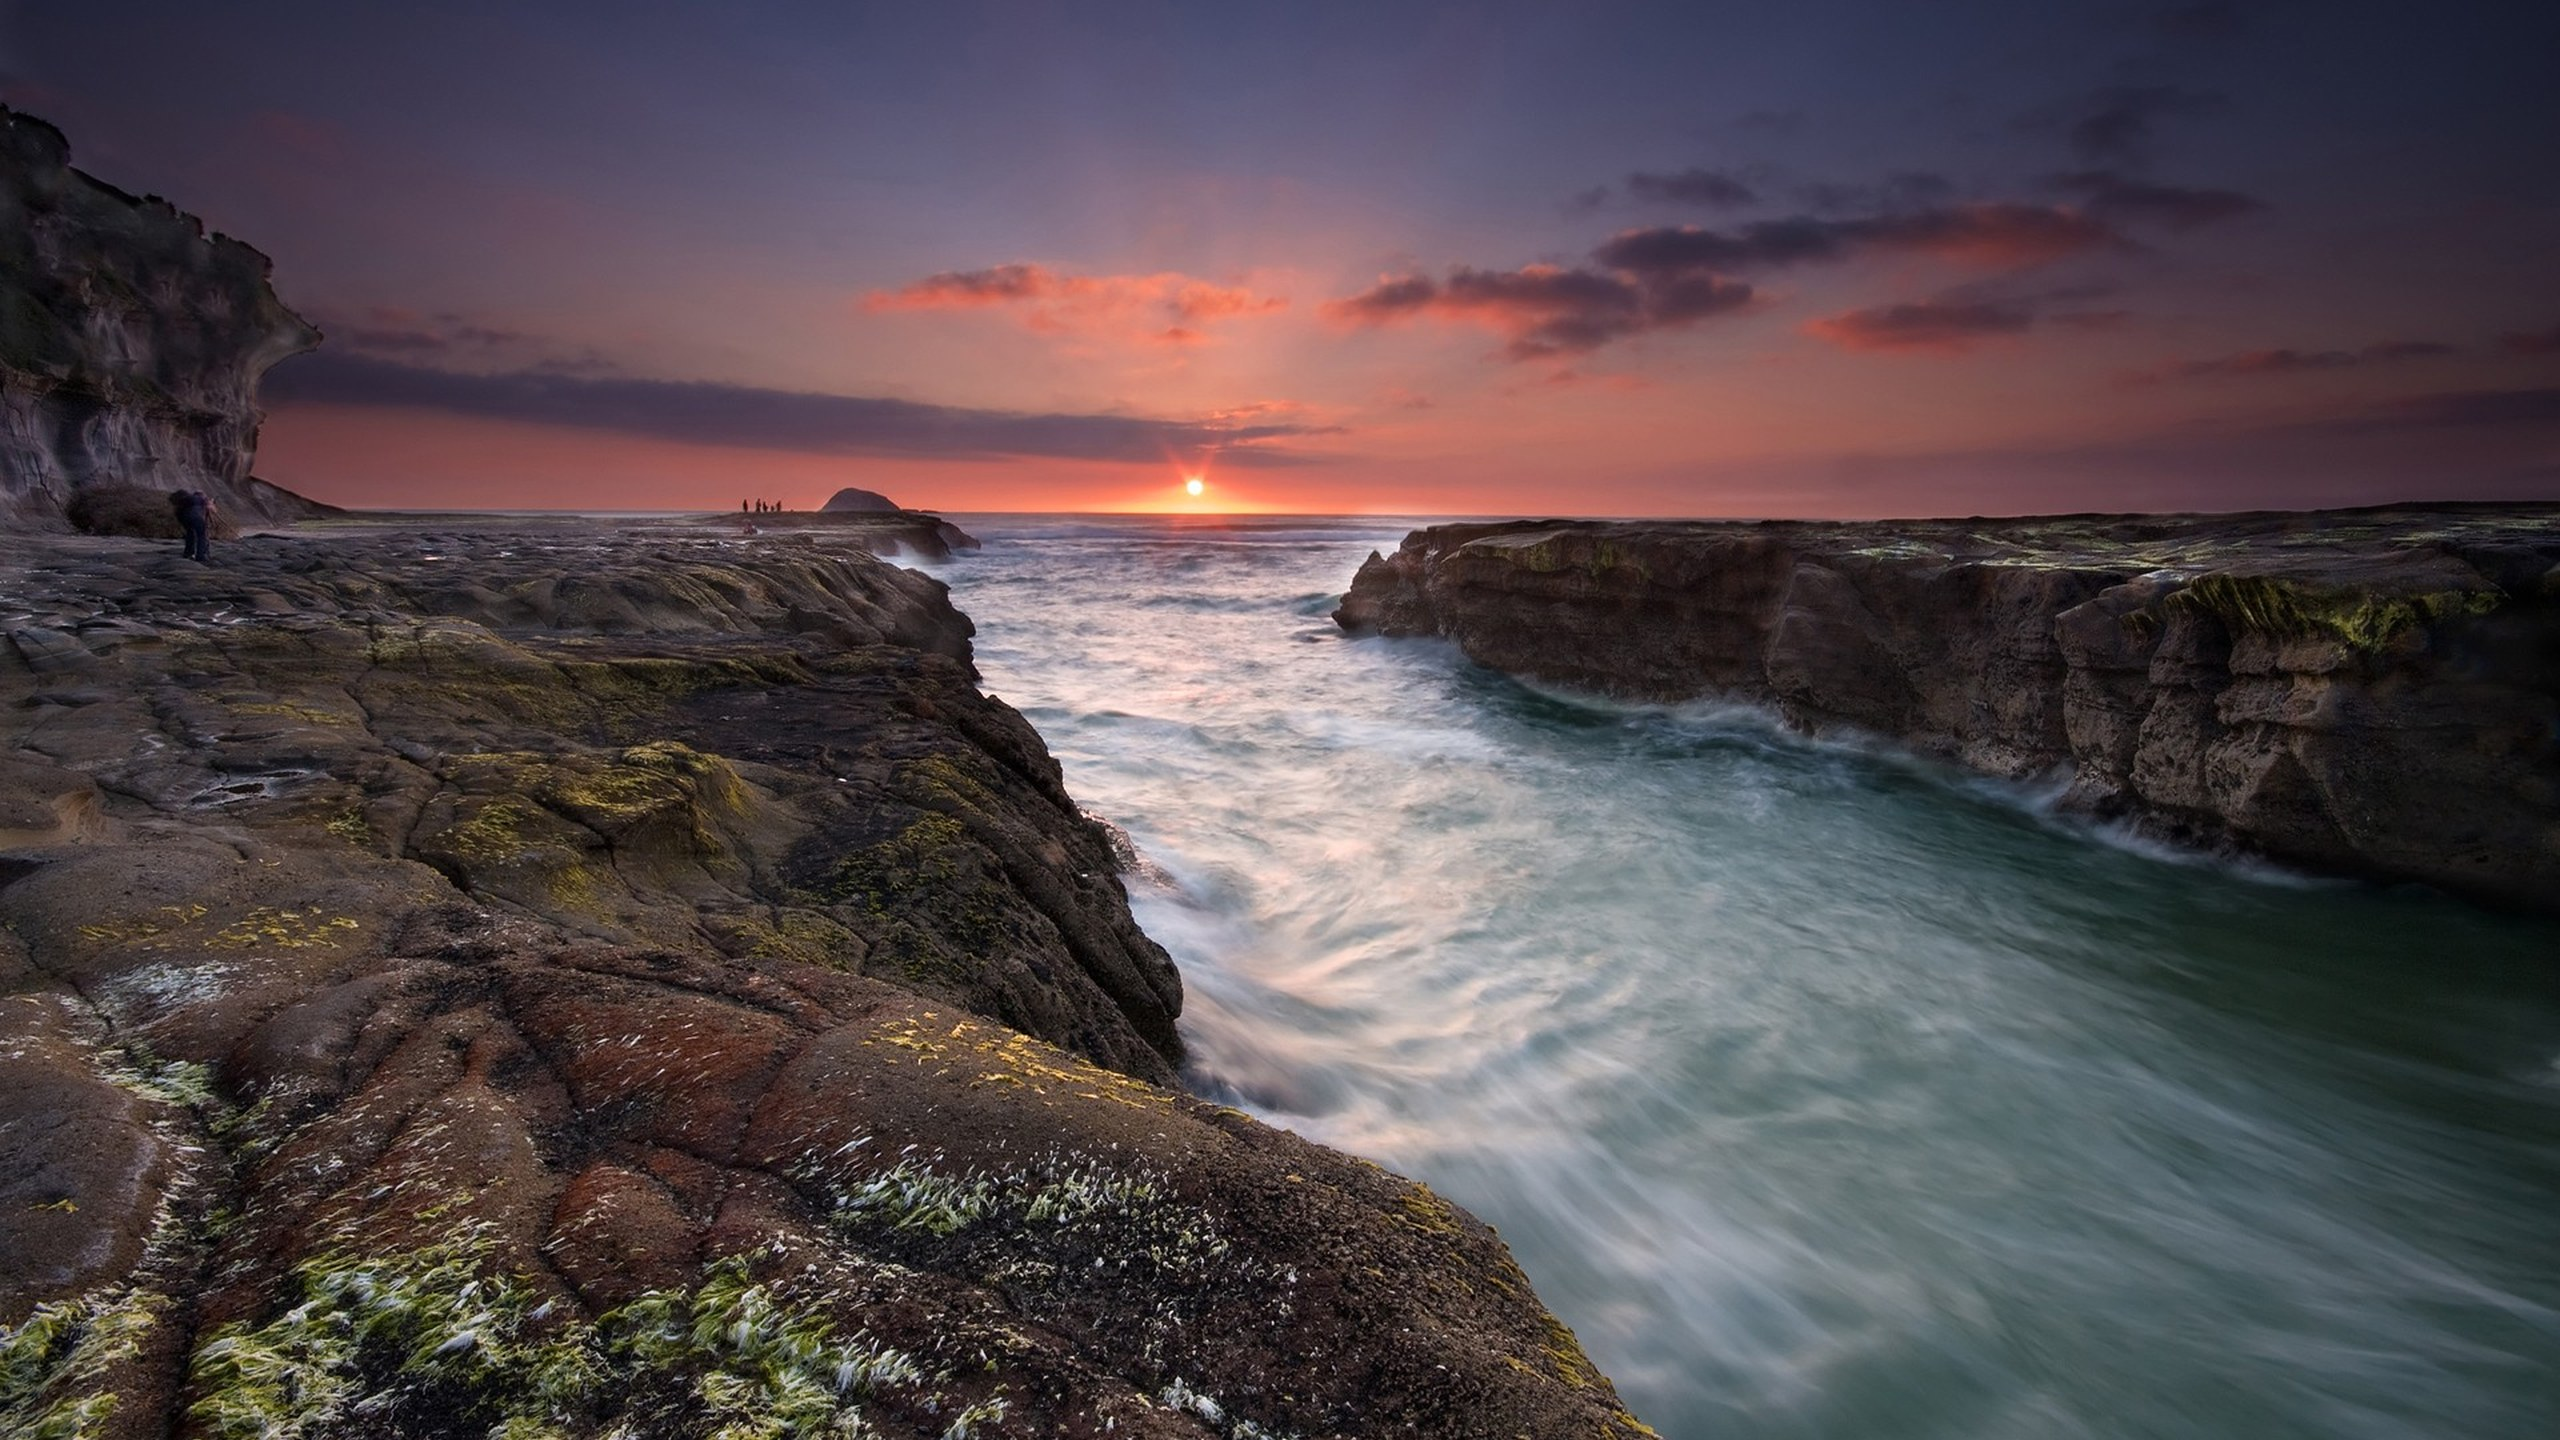
\includegraphics[width=0.48\textwidth]{testimage3.jpg}
        \label{subfig:testimage3}
    }
    \vfill
    \subfloat[]{
        
\includegraphics[width=0.48\textwidth]{testimage4.jpg}
        \label{subfig:testimage4}
    }
    \caption{这是另一组风景图。(a)风景图3;(b)风景图4。}
    \label{fig:group2}
\end{figure}
\vspace{10pt}

这是\subfigref{subfig:testimage3},这是\subfigref{subfig:testimage4},这是\figref{fig:group2}。
